\title{Getting started with the E. Coli Whole Cell Model on Sherlock: A Brief Tutorial}


\documentclass[12pt]{article}

\usepackage{graphicx}
\usepackage[parfill]{parskip}
\usepackage{listings}
\usepackage{color}
\usepackage{underscore}

\definecolor{dkgreen}{rgb}{0,0.6,0}
\definecolor{gray}{rgb}{0.5,0.5,0.5}
\definecolor{mauve}{rgb}{0.58,0,0.82}

\lstset{frame=tb,
  language=Python,
  aboveskip=3mm,
  belowskip=3mm,
  showstringspaces=false,
  columns=flexible,
  basicstyle={\small\ttfamily},
  numbers=none,
  numberstyle=\tiny\color{gray},
  keywordstyle=\color{blue},
  commentstyle=\color{dkgreen},
  stringstyle=\color{mauve},
  breaklines=true,
  breakatwhitespace=true,
  tabsize=3
}

\begin{document}
\maketitle

\section{Basics}

This document is an introduction to running the whole-cell E.coli model on the Sherlock computing cluster. In addition to setup and a tutorial on modifying the model, it will include a brief primer on some of model knowledge base fitting in later sections.
\par
First a basic note on file locations. The knowledge base and the code that fits the knowledge base is located in the wcEcoli/reconstruction/ecoli/ directory. The input information files are in wcEcoli/reconstruction/ecoli/flat, and the code that loads it into an object is in knowledge\_base\_raw.py.
\par

Processes are located in wcEcoli/models/ecoli/processes/. Each process represents one part of the cell's function, and they are modeled separately in short time steps and then the results of each time step are integrated between modules before initiating the next time step. RNA polymerase elongation is the processed used below as an example in this tutorial. Other processes include translation elongation, transciption initiation, and metabolism.
\par
Each process has three components: initialize (called only once at the beginning of a simulation), calculateRequest (called at the beginning of each timestep), and evolveState (called after resources are allocated at each timestep).
\par
\emph{In initialize}: get needed parameters from the knowledge base, get views of bulk and unique molecules (bulk molecules are “indistinguishable” from each other, e.g. inactive RNAP molecules, unique molecules can be distinguished from each other, e.g. active RNAP molecules are each assigned to a specific transcript), create a view so that you can get counts, change counts, and change properties.
\par
\emph{In calculateRequest}: request the resources that you want for that timestep (don’t request all unless you are certain that another process doesn’t need this resource as well, don’t forget about metabolism).
\par
\emph{In evolveState}: resources have been allocated, perform the process, update counts, and update masses (mass must be conserved between steps).
\par
If you need new output, you must write this out as a listener. Listeners are programs which record information during the simulation. To add a listener, add the file to wcEcoli/models/ecoli/listeners/, and both add an import statement and add the listener to \_listenerClasses in wcEcoli/models/ecoli/sim/simulation.py.
\par
To change the cell’s initial conditions, change wcEcoli/models/ecoli/sim/initial\_conditions.py
\par

\section{Setup}
\label{sec:setup}

This tutorial assumes you have setup access to the Sherlock cluster. If necessary before following the proceeding steps, do the following setup:

\begin{enumerate}
\item Email the research computing staff at research-computing-support@stanford.edu, and cc Professor Covert. Request access to the Sherlock cluster, and ask Professor Covert to confirm your request in the email.

\item Follow the setup instructions for logging in to Sherlock on
\linebreak
http://covert.stanford.edu/computational\_resources/sherlock/home/.

\item Follow all setup instructions in the wcEcoli/README.md file (also on the web at https://github.com/CovertLab/wcEcoli/blob/master/README.md).
\end{enumerate}

Once done with setup and these basic tutorials on Sherlock and the cluster, return to here to complete the example.



\section{Example: varying trascription rate}

\subsection{Background}

Genes encoding for stable RNA are transcribed at a faster rate in E. Coli. In the model (prior to this tutorial), all genes were transcribed at the same rate of 42nt/s. In this tutorial, we will change the model so that genes for rRNA and tRNA are transcribed at 80nt/s while everything else is still transcribed at 42nt/s. 
\par

The code has inevitably evolved since I wrote this tutorial, so let’s get on the same page by going back to an older version of the code. Let’s do this tutorial on a new branch. cd into your wcEcoli directory and type:

\lstset{language=bash}
\begin{lstlisting}
git checkout -b tutorial wholecell-tutorial
\end{lstlisting}

We need to make sure the output from the model goes to the SCRATCH filesystem (whcih is larger) rather than SHERLOCK\_HOME. We'll need to make a symbolic link between the output directory of your wcEcoli directory and a directory in SCRATCH. Within your wcEcoli diretory, there should be a folder named out/. The model puts its outputput in this folder, so we can basically tell the computer to send anything placed in this folder to SCRATCH instead.

First go to SCRATCH and create a folder in which to place the output. Run the following command:

\lstset{language=bash}
\begin{lstlisting}
cd $SCRATCH
\end{lstlisting}

Now make a directory to hold the output. You can call it whatever you want, here is one option:

\lstset{language=bash}
\begin{lstlisting}
mkdir wcEcoli_out
\end{lstlisting}

Return to wcEcoli home with

\lstset{language=bash}
\begin{lstlisting}
cd $HOME/wcEcoli
\end{lstlisting}

To create the symbolic link, we first need to delete the existing out/ directory. Do this with:

\lstset{language=bash}
\begin{lstlisting}
rmdir out/
\end{lstlisting}

Now run this command to make the symbolic link. Change the name of the directory to the one you made on SCRATCH if it's different.

\lstset{language=bash}
\begin{lstlisting}
ln -s $SCRATCH/wcEcoli_out out
\end{lstlisting}


Now let's try running the unmodified model to make sure it works. From within your wcEcoli directory in Sherlock, queue up a simple run of the model.

\lstset{language=bash}
\begin{lstlisting}
DESC="Tutorial run, starting code with unmodified parameters." python runscripts/fw_queue.py
\end{lstlisting}

Run the tasks in the queue until finished:

\begin{lstlisting}
rlaunch rapidfire
\end{lstlisting}



\subsection{Add a new parameter to the model}

First, let’s add a new elongation rate to the knowledge base. In reconstruction/ecoli/flat is a tsv called growthRateDependentParameters.tsv. Add a new column for the fast rna polymerase rate (estimate that it is double the normal rate). The normal rate at each growth rate is stored in the column 'rnaPolymeraseElongationRate'. This command will generate the file with the new column appended, or edit the file in a different way if desired.

\pagebreak

\begin{lstlisting}
awk '{if(NR==1){print $0 "\t" "rnaPolymeraseElongationRateFast (units.nt/units.min)"}else{print $0 "\t" ($9*2)}}' growthRateDependentParameters.tsv > temp && mv temp growthRateDependentParameters.tsv  
\end{lstlisting}

Alternatively, you could open the .tsv file in a spreadsheet editor and add the new column by hand.

To check that the parameter was added, examine the knowledge base object in ipython.

\lstset{language=Python}
\begin{lstlisting}
ipython
import reconstruction.ecoli.knowledge_base_raw as kbr
kb=kbr.KnowledgeBaseEcoli()
kb.growthRateDependentParameters[0]
\end{lstlisting}

You should see the 'rnaPolymeraseElongationRateFast': 78 [nucleotide/min]' entry in the resulting dictionary.

\subsection{Create a new process}

Let’s split the transcript elongation process into a slow process and a fast process. Go to models/ecoli/processes/ :

\lstset{language=bash}
\begin{lstlisting}
cd models/ecoli/processes/

cp transcript_elongation.py transcript_elongation_fast.py

mv transcript_elongation.py transcript_elongation_slow.py
\end{lstlisting}

Now we need to add these processes to the simulation, so that they actually get called. Let’s go back to the wcEcoli directory. Open models/ecoli/sim/simulation.py and change line 19 to read: 

\lstset{language=Python}
\begin{lstlisting}
from models.ecoli.processes.transcript_elongation_slow import TranscriptElongationSlow
\end{lstlisting}

Then add a line just under this:

\begin{lstlisting}
from models.ecoli.processes.transcript_elongation_fast import TranscriptElongationFast
\end{lstlisting}

Under process classes, add TranscriptElongationFast and change TranscriptElongation to TranscriptElongationSlow. \_processClasses should now look like this:


\begin{lstlisting}
        _processClasses = (
                Metabolism,
                RnaDegradation,
                TranscriptInitiation,
                TranscriptElongationSlow,
                TranscriptElongationFast,
                PolypeptideInitiation,
                PolypeptideElongation,
                Replication,
                ProteinDegradation,
                Complexation,
                AtpUsage
                )
\end{lstlisting}

\subsection{Change the model output}

Now let’s change the listeners to record output from these new processes. We write data to listeners, and the listener is responsible for recording the data to the file, as well as transforming it as necessary (calculating averages, for example). The transcription submodels write to three listeners: GrowthLimits, RnapData, and TranscriptElongationListener. We need to make several changes in order to correctly log transcription data. The fast and slow transcription submodels need to both write to the same listener attributes, so we need to set them up to add data together, rather than overwriting one another's output.

First, we need to update the listeners to zero out the relevant attributes each time step, so that we can add to them from each model. Open models/ecoli/listeners/growth_limits.py and add the following lines to the end of tableAppend(...), at line 100:

\lstset{language=Python}
\begin{lstlisting}
self.ntpRequestSize = np.zeros(len(self.ntpIds), np.float64)
self.ntpAllocated = np.zeros(len(self.ntpIds), np.float64)
self.ntpUsed = np.zeros(len(self.ntpIds), np.float64)
\end{lstlisting}

We need to make two changes to models/ecoli/listeners/rnap_data.py. At line 73, update the lines that read:
\lstset{language=Python}
\begin{lstlisting}
self.rnapStalls = np.zeros(0, np.int64)
self.ntpCountInSequence = np.zeros(21, np.int64)
self.ntpCounts = np.zeros(21, np.int64)
\end{lstlisting}

To read:
\lstset{language=Python}
\begin{lstlisting}
self.rnapStalls = np.empty(0, np.int64)
self.ntpCountInSequence = np.empty(0, np.int64)
self.ntpCounts = np.empty(0, np.int64)
\end{lstlisting}

This initialises some arrays we'll be writing to to be completely empty, which allows us to append to them without having a bunch of leading data we don't want. Next, we reset the relevant attributes as in GrowthLimits. Add the following to the bottom of tableAppend(...), at line 119:
\lstset{language=Python}
\begin{lstlisting}
self.rnapStalls = np.empty(0, np.int64)
self.ntpCountInSequence = np.empty(0, np.int64)
self.ntpCounts = np.empty(0, np.int64)
self.expectedElongations = 0
self.actualElongations = 0
self.didTerminate = 0
self.terminationLoss = 0
\end{lstlisting}

Finally, we need to update models/ecoli/listeners/transcript_elongation_listener.py. Add to the bottom of tableAppend(...) at line 47:
\lstset{language=Python}
\begin{lstlisting}
self.countRnaSynthesized = np.zeros(self.countRnaSynthesized.shape, self.countRnaSynthesized.dtype)
\end{lstlisting}

\subsection{Modify a process}

Now let’s modify the new processes. Open models/ecoli/processes/transcript\_elongation\_slow.py and change all references of TranscriptElongation to TranscriptElongationSlow.

Next create a Boolean vector that is True at the indices of transcripts that should be elongated at the slow rate and False at the indices of transcripts that should be elongated at the fast rate. In the initialize function add the following line (after line 70):

\lstset{language=Python}
\begin{lstlisting}
self.slowRnaBool = ~(sim_data.process.transcription.rnaData["isRRna5S"] | sim_data.process.transcription.rnaData["isRRna16S"] | sim_data.process.transcription.rnaData["isRRna23S"] | sim_data.process.transcription.rnaData["isTRna"])
\end{lstlisting}

“isRRna5S”, “isRRna16S”, “isRRna23S”, and “isTRna” are properties of rnaData, which is found in the simulation data set (sim_data). These are vectors of Boolean values. The tilde inverts the boolean value, so this creates a vector that is False for all 5S rRNA, 16S rRNA, 23S rRNA, and tRNA, and True for everything else.
Now let’s change the view onto the active rna polymerases to a view onto only the active rna polymerases that are on transcripts that should be elongated at the slow rate. Change the definition of self.activeRnaPolys (line 75) to read:

\begin{lstlisting}
    self.activeRnaPolys = self.uniqueMoleculesView(
      'activeRnaPoly',
      rnaIndex = ("in", np.where(self.slowRnaBool)[0]))
\end{lstlisting}

Next, we need to update our writes to the listeners to increment or append, rather than overwrite, the attributes that are updated. First, add a new import at the top of the file (around line 25):
\begin{lstlisting}
from wholecell.listeners.listener import WriteMethod
\end{lstlisting}

Second, we need to change our calls to writeToListener(...) to either increment (in the case of numeric attributes), or append (in the case of arrays), rather than overwriting. Modify all of the writeToListener(...) calls to have a new parameter at the end:  WriteMethod.increment, except for the writes to rnapStalls, ntpCountInSequence, and ntpCounts, which instead should have WriteMethod.append. Overall, the lines should look like the following (although in the file they are scattered around a bit):
\begin{lstlisting}
self.writeToListener("GrowthLimits", "ntpRequestSize", maxFractionalReactionLimit * sequenceComposition, WriteMethod.increment)

self.writeToListener("GrowthLimits", "ntpAllocated", self.ntps.counts(), WriteMethod.increment)

self.writeToListener("TranscriptElongationListener", "countRnaSynthesized", terminatedRnas, WriteMethod.increment)

self.writeToListener("GrowthLimits", "ntpUsed", ntpsUsed, WriteMethod.increment)
self.writeToListener("RnapData", "rnapStalls", rnapStalls, WriteMethod.append)
self.writeToListener("RnapData", "ntpCountInSequence", ntpCountInSequence, WriteMethod.append)
self.writeToListener("RnapData", "ntpCounts", ntpCounts, WriteMethod.append)
self.writeToListener("RnapData", "expectedElongations", expectedElongations.sum(), WriteMethod.increment)
self.writeToListener("RnapData", "actualElongations", sequenceElongations.sum(), WriteMethod.increment)
self.writeToListener("RnapData", "didTerminate", didTerminate.sum(), WriteMethod.increment)
self.writeToListener("RnapData", "terminationLoss", (terminalLengths - transcriptLengths)[didTerminate].sum(), WriteMethod.increment)
\end{lstlisting}

This is all we need to change in this file. Now let’s open the fast transcript elongation file models/ecoli/processes/transcript\_elongation\_fast.py. Similarly to what we did in the slow elongation file, let’s change all references of TranscriptElongation to TranscriptElongationFast.

Now, let’s create the opposite of the Boolean vector that we created in the transcript\_elongation\_slow. In the initialize function add the following line (after line 70):

\lstset{language=Python}
\begin{lstlisting}
self.fastRnaBool = sim_data.process.transcription.rnaData["isRRna5S"] | sim_data.process.transcription.rnaData["isRRna16S"] | sim_data.process.transcription.rnaData["isRRna23S"] | sim_data.process.transcription.rnaData["isTRna"]
\end{lstlisting}

Now let’s change the view onto the active rna polymerases to a view onto only the active rna polymerases that are on transcripts that should be elongated at the fast rate (line 75):

\begin{lstlisting}
                 self.activeRnaPolys = self.uniqueMoleculesView(
                         'activeRnaPoly',
                         rnaIndex = ("in", np.where(self.fastRnaBool)[0])
                         )
\end{lstlisting}

Finally, let’s change the elongation rate. Change line 59 to read:

\begin{lstlisting}
self.elngRate = kb.rnaPolymeraseElongationRateFast.asNumber(units.nt / units.s) * self.timeStepSec
\end{lstlisting}

Update the writeToListener(...) lines to match the changes you made in TranscriptElongationSlow, above. Now data from both submodels will be recorded in the whole cell output.

\par
Now we can run a simulation and rRNA and tRNA would be transcribed at the new fast rate, while everything else was transcribed at the same slow rate before. Follow these steps to run the new simulation code:
\par
Queue up the tasks in fireworks:

\lstset{language=bash}
\begin{lstlisting}
DESC="Tutorial run, adding different RNA polymerization rate for r- and t- RNAs." python runscripts/fw_queue.py
\end{lstlisting}

Run the tasks in the queue until finished:

\begin{lstlisting}
rlaunch rapidfire
\end{lstlisting}

To check for the success of your simulation, open the /out/ folder, and the folder timestamped to the simulation just run, then click through to the output plots. Specifically look at the rnapActiveFraction plot. This should be around 20\%. Is it? Also look at the massFractionSummary plot. Does everything roughly double in one cell cycle? If not, why might that be?

\subsection{Changing the fitting}

Even though we've changed the model, the simulation will be initialized the same way as before. This is a problem because before running a simulation, we need to fit several initial parameters including the initial counts of RNA polymerases and the activation rate of the RNA polymerases. Because some things are now being transcribed at a faster rate, we should need fewer RNA polymerases to make the same number of transcripts. Additionally, if some things are being transcribed more quickly, then RNA polymerases will be inactivating more quickly. In order to maintain a constant ratio of active to inactive RNA polymerases (experimentally shown to be around 20\%), the activation rate must also increase now. 

\par

We calculate the number of RNA polymerases that we need initially by writing an equation for the rate of change of some RNA $R_i$ (rate of synthesis – rate of degradation = rate of dilution due to growth):

$$
\frac{d R_i}{dt} = \frac{k_{elong}}{L_i}P_i(t) - \frac{\ln(2)}{h_i}R_i(t) = \frac{\ln(2)}{\tau_d}R_i(t)
$$


$L_i$ is the length of transcript $i$; $P_i$ is the number of RNA polymerases actively transcribing $R_i$ at time $t$; $h_i$ is the half life of $R_i$; $\tau_d$ is the length of the cell cycle; $k_{elong}$ is the transcript elongation rate. Right now this is a constant value for all transcripts. We want to change this to be different for rRNA and tRNA. Let’s change this in the code. Open the file reconstruction/ecoli/fit_sim_data_1.py and go to the setRNAPCountsConstrainedByPhysiology function. This is what we need to change. Let’s add the Boolean vectors for fast and slow transcripts. Right at the beginning of this function definition (after the docstring), add these two lines:

\lstset{language=Python}
\begin{lstlisting}
fastRnaBool = kb.process.transcription.rnaData["isRRna5S"] | kb.process.transcription.rnaData["isRRna16S"] | kb.process.transcription.rnaData["isRRna23S"] | kb.process.transcription.rnaData["isTRna"]
slowRnaBool = ~fastRnaBool
\end{lstlisting}

Let’s break up the calculation of nActiveRnapNeeded into nActiveRnapNeededforFast and nActiveRnapNeededforSlow. Change the nActiveRnapNeeded calculation to read:

\begin{lstlisting}
nActiveRnapNeededforSlow = calculateMinPolymerizingEnzymeByProductDistributionRNA(
    rnaLengths[slowRnaBool], 
    sim_data.growthRateParameters.rnaPolymeraseElongationRate, 
    rnaLossRate[slowRnaBool])
\end{lstlisting}

Add a line under this for the calculation for the fast transcripts:

\begin{lstlisting}
nActiveRnapNeededFast = calculateMinPolymerizingEnzymeByProductDistributionRNA(
    rnaLengths[fastRnaBool], 
    sim_data.growthRateParameters.rnaPolymeraseElongationRateFast, 
    rnaLossRate[fastRnaBool])
\end{lstlisting}

Below this, add a line to calculate the total number of RNA polymerases needed:

\begin{lstlisting}
nActiveRnapNeeded = nActiveRnapNeededforFast + nActiveRnapNeededforSlow
\end{lstlisting}

Now let’s change the calculation of the RNA polymerase activation rate. In the model, an RNA polymerase can either be active or inactive:

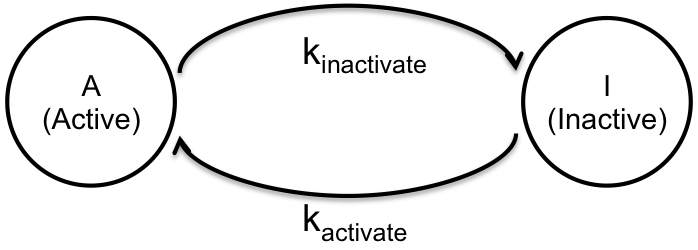
\includegraphics{img.png}


To calculate the rate of activation, $k_{activate}$, we write an equation for the rate of change of the number of RNAP active at steady state:

$$
\frac{dA}{dt}=k_{activate}I - k_{inactivate}A=0
$$

This gives us that

$$
k_{activate} = k_{inactivate}\frac{A}{I}
$$


We know from experiments the fraction of RNA polymerases that are active, $f_{active}$:

$$
f_{active}=\frac{A}{A+I}
$$

Using that 

$$
f_{active} = 1 - f_{inactive}
$$

We can rearrange and solve for the rate of activation:

$$
k_{activate}=k_{inactivate}\left(\frac{f_{active}}{1-f_{active}} \right)
$$

We can calculate the rate of inactivation from the elongation rate, the transcript lengths, and the synthesis probabilities:

$$
k_{inactivate}=\frac{k_{elong}}{L_i}\cdot\frac{1}{p_{synth}}
$$

We want to change the elongation rate to be a vector, rather than a constant:

$$
k_{inactivate}=\frac{k_{elong,i}}{L_i}\cdot \frac{1}{p_{synth}}
$$

Now let’s do this in the code. In reconstruction/ecoli/fitkb1.py, in the fitRNAPolyTransitionRates function (on line 483), at the top add the following lines. The tilde operator inverts the booleans.

\begin{lstlisting}
fastRnaBool = (
    sim_data.process.transcription.rnaData["isRRna5S"] |
    sim_data.process.transcription.rnaData["isRRna16S"] |
    sim_data.process.transcription.rnaData["isRRna23S"] |
    sim_data.process.transcription.rnaData["isTRna"])
slowRnaBool = ~fastRnaBool
\end{lstlisting}

Now, delete the elngRate definition (elngRate = kb.rnaPolymeraseElongationRate) and add an elongation rate vector:

\begin{lstlisting}
elngRateVector = slowRnaBool * sim_data.growthRateParameters.rnaPolymeraseElongationRate + fastRnaBool * sim_data.growthRateParameters.rnaPolymeraseElongationRateFast
\end{lstlisting}

Delete the calculation of averageTranscriptLength and expectedTerminationRate and add the following three lines:

\begin{lstlisting}
expectedTranscriptionTime = rnaLengths/elngRateVector

weightedExpectedTranscriptionTime = units.dot(synthProb, expectedTranscriptionTime)

expectedTerminationRate = 1/weightedExpectedTranscriptionTime
\end{lstlisting}

We’re done editing this file now. Now the fitting of the initial number of RNA polymerases and the activation rate is fixed. 




\subsection{Running simulations}

Now we can run some simulations. Be sure to complete the setup section (\ref{sec:setup}) if you haven't already.
\par
First log in to a sherlock node. Replace 'username' with your username in the command below:

\lstset{language=bash}
\begin{lstlisting}
ssh username@sherlock
\end{lstlisting}

Now log in to a non-login node, so that the simulation can be run in interactive mode (running in interactive mode on a login node can result in getting booted from the cluster). These nodes are covert-lab specific and it's ok to do more serious computation on them.

\begin{lstlisting}
srun -p mcovert --ntasks-per-node=1 --time=12:00:00 --pty bash
\end{lstlisting}

Now prepare the fireworks queue with your simulation task. 
\par
Once setup is complete, change the DESC description text as desired, and run:

\begin{lstlisting}
DESC="Tutorial run, adding different RNA polymerization rate for r- and t- RNAs." python runscripts/fw_queue.py
\end{lstlisting}

Now the simulation task is queued up in fireworks and can be launched via:

\begin{lstlisting}
rlaunch rapidfire
\end{lstlisting}

After about a minute, this should start producing output looking something like this:

\begin{lstlisting}
[mpaull@sh-8-31 ~/wcEcoli]$ rlaunch rapidfire
2015-06-23 19:09:29,106 INFO Hostname/IP lookup (this will take a few seconds)
2015-06-23 19:09:29,814 INFO Created new dir /home/mpaull/wcEcoli/launcher_2015-06-24-02-09-29-810292
2015-06-23 19:09:29,817 INFO Launching Rocket
2015-06-23 19:09:32,285 INFO RUNNING fw_id: 12 in directory: /home/mpaull/wcEcoli/launcher_2015-06-24-02-09-29-810292
2015-06-23 19:09:32,289 INFO Task started: {{wholecell.fireworks.firetasks.initKb.InitKbTask}}.
Tue Jun 23 19:09:32 2015: Instantiating unfit knowledgebase
Tue Jun 23 19:09:32 2015: Saving unfit knowledgebase
2015-06-23 19:09:32,292 INFO Task completed: {{wholecell.fireworks.firetasks.initKb.InitKbTask}} 
2015-06-23 19:09:34,950 INFO Rocket finished
2015-06-23 19:09:35,328 INFO Created new dir /home/mpaull/wcEcoli/launcher_2015-06-24-02-09-35-326470
2015-06-23 19:09:35,330 INFO Launching Rocket
2015-06-23 19:09:37,772 INFO RUNNING fw_id: 10 in directory: /home/mpaull/wcEcoli/launcher_2015-06-24-02-09-35-326470
2015-06-23 19:09:37,775 INFO Task started: {{wholecell.fireworks.firetasks.symlink.SymlinkTask}}.
Tue Jun 23 19:09:37 2015: Creating symlink
2015-06-23 19:09:37,777 INFO Task completed: {{wholecell.fireworks.firetasks.symlink.SymlinkTask}} 
2015-06-23 19:09:40,154 INFO Rocket finished
2015-06-23 19:09:40,531 INFO Created new dir /home/mpaull/wcEcoli/launcher_2015-06-24-02-09-40-530368
2015-06-23 19:09:40,533 INFO Launching Rocket
2015-06-23 19:09:42,981 INFO RUNNING fw_id: 9 in directory: /home/mpaull/wcEcoli/launcher_2015-06-24-02-09-40-530368
2015-06-23 19:09:42,984 INFO Task started: {{wholecell.fireworks.firetasks.fitKb.FitKbTask}}.
Tue Jun 23 19:09:42 2015: Fitting knowledgebase (Level 1)
 \end{lstlisting}



\hfill \break
\hfill \break



Then once the actual simulation starts, you will see:

\hfill \break
\hfill \break



\begin{lstlisting}
Tue Jun 23 19:10:13 2015: Running simulation
Time (s)  Dry mass     Dry mass      Protein          RNA     Expected
              (fg)  fold change  fold change  fold change  fold change
========  ========  ===========  ===========  ===========  ===========
       0    245.19        1.000        1.000        1.000        1.000
Warning - converting 'reactionIDs' attribute from ndarray to list for JSON serialization.
       1    245.27        1.000        1.000        1.000        1.000
       2    245.20        1.000        1.000        1.000        1.000
       3    244.50        0.997        1.000        1.000        1.001
       4    244.52        0.997        1.000        1.000        1.001
       5    244.58        0.998        1.001        1.001        1.001
       6    244.63        0.998        1.001        1.002        1.001
       7    244.64        0.998        1.001        1.003        1.001
       8    244.63        0.998        1.001        1.004        1.002
       9    244.73        0.998        1.001        1.005        1.002
      10    244.79        0.998        1.002        1.007        1.002
      11    244.87        0.999        1.002        1.008        1.002
      12    244.96        0.999        1.002        1.010        1.002
      13    245.08        1.000        1.002        1.012        1.003
      14    245.10        1.000        1.002        1.014        1.003
      15    245.21        1.000        1.003        1.016        1.003
      16    245.32        1.001        1.003        1.018        1.003
      17    245.41        1.001        1.003        1.021        1.003
      18    245.49        1.001        1.003        1.023        1.003
      19    245.59        1.002        1.003        1.026        1.004
      20    245.69        1.002        1.004        1.028        1.004
      21    245.79        1.002        1.004        1.031        1.004
      22    245.89        1.003        1.004        1.034        1.004
      23    245.95        1.003        1.004        1.037        1.004
      24    246.04        1.003        1.005        1.040        1.005
      25    246.14        1.004        1.005        1.043        1.005
      26    246.23        1.004        1.005        1.046        1.005
      27    246.33        1.005        1.005        1.049        1.005
      28    246.41        1.005        1.005        1.052        1.005
      29    246.51        1.005        1.006        1.056        1.006
      30    246.60        1.006        1.006        1.059        1.006
      31    246.70        1.006        1.006        1.062        1.006
      32    246.79        1.007        1.006        1.066        1.006
      33    246.88        1.007        1.006        1.069        1.006
      34    246.98        1.007        1.007        1.073        1.007
      35    247.07        1.008        1.007        1.076        1.007
      36    247.16        1.008        1.007        1.079        1.007
      37    247.26        1.008        1.007        1.083        1.007
      38    247.35        1.009        1.007        1.087        1.007
      39    247.43        1.009        1.008        1.090        1.008
      40    247.52        1.010        1.008        1.094        1.008
      41    247.61        1.010        1.008        1.098        1.008
      42    247.70        1.010        1.008        1.101        1.008
      43    247.79        1.011        1.008        1.105        1.008
      44    247.88        1.011        1.009        1.109        1.009
      45    247.97        1.011        1.009        1.113        1.009
      46    248.05        1.012        1.009        1.116        1.009
      47    248.14        1.012        1.009        1.120        1.009
      48    248.23        1.012        1.009        1.124        1.009
      49    248.31        1.013        1.010        1.128        1.009
\end{lstlisting}

\hfill \break
\hfill \break

This will take a few minutes to run. At the end you can find the output in the out/timestamp directory (timestamp obviously replaced with the actual timestamp of when you started the simulation). Look at the plots in the /wcEcoli/out/20150623.190922.827654/wildtype\_000000/000000/generation\_00
0000/000000/plotOut directory (replacing the timestamp directory with your own timestamped directory name).

\end{document}